\section{Lý do chọn đề tài}

Hiện nay, phần lớn các bãi giữ xe đều sử dụng thẻ từ, Rfid hoặc thẻ giấy để kiểm soát phương tiện. Khi xe ra vào, người dùng phải quét thẻ tại trạm kiểm soát để hệ thống xác thực và mở cổng. Ví dụ trong trường đại học Giao Thông Vận Tải Thành phố Hồ Chí Minh sử dụng thẻ từ để quét biển số xe được nhóm thu thập hình ảnh về thẻ xe và máy quét thẻ của bãi đỗ xe dưới đây.

\begin{figure}[H]
    \centering
    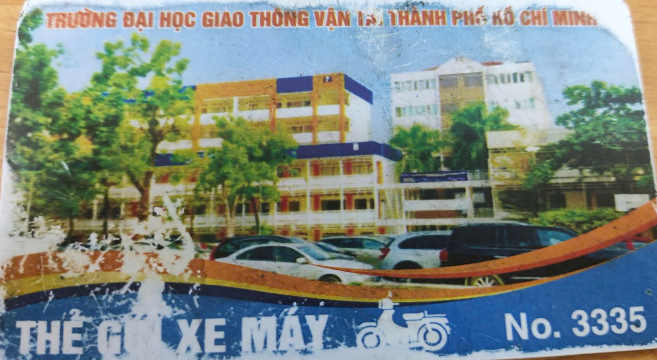
\includegraphics[width=1\textwidth]{graphics/main/chapter1/parking_card_front.png}
    \caption{Hình mặt trước thẻ giữ xe}
    \label{fig:thegiu-xe}
\end{figure}

\begin{figure}[H]
    \centering
    
\includegraphics[width=1\textwidth]{graphics/main/chapter1/parking_card_back.png}
    \caption{Hình mặt sau thẻ giữ xe}
    \label{fig:thegiu-xe}
\end{figure}
